% Options for packages loaded elsewhere
\PassOptionsToPackage{unicode}{hyperref}
\PassOptionsToPackage{hyphens}{url}
%
\documentclass[
  man,floatsintext,draftall]{apa6}
\usepackage{amsmath,amssymb}
\usepackage{lmodern}
\usepackage{iftex}
\ifPDFTeX
  \usepackage[T1]{fontenc}
  \usepackage[utf8]{inputenc}
  \usepackage{textcomp} % provide euro and other symbols
\else % if luatex or xetex
  \usepackage{unicode-math}
  \defaultfontfeatures{Scale=MatchLowercase}
  \defaultfontfeatures[\rmfamily]{Ligatures=TeX,Scale=1}
\fi
% Use upquote if available, for straight quotes in verbatim environments
\IfFileExists{upquote.sty}{\usepackage{upquote}}{}
\IfFileExists{microtype.sty}{% use microtype if available
  \usepackage[]{microtype}
  \UseMicrotypeSet[protrusion]{basicmath} % disable protrusion for tt fonts
}{}
\makeatletter
\@ifundefined{KOMAClassName}{% if non-KOMA class
  \IfFileExists{parskip.sty}{%
    \usepackage{parskip}
  }{% else
    \setlength{\parindent}{0pt}
    \setlength{\parskip}{6pt plus 2pt minus 1pt}}
}{% if KOMA class
  \KOMAoptions{parskip=half}}
\makeatother
\usepackage{xcolor}
\usepackage{graphicx}
\makeatletter
\def\maxwidth{\ifdim\Gin@nat@width>\linewidth\linewidth\else\Gin@nat@width\fi}
\def\maxheight{\ifdim\Gin@nat@height>\textheight\textheight\else\Gin@nat@height\fi}
\makeatother
% Scale images if necessary, so that they will not overflow the page
% margins by default, and it is still possible to overwrite the defaults
% using explicit options in \includegraphics[width, height, ...]{}
\setkeys{Gin}{width=\maxwidth,height=\maxheight,keepaspectratio}
% Set default figure placement to htbp
\makeatletter
\def\fps@figure{htbp}
\makeatother
\setlength{\emergencystretch}{3em} % prevent overfull lines
\providecommand{\tightlist}{%
  \setlength{\itemsep}{0pt}\setlength{\parskip}{0pt}}
\setcounter{secnumdepth}{-\maxdimen} % remove section numbering
% Make \paragraph and \subparagraph free-standing
\ifx\paragraph\undefined\else
  \let\oldparagraph\paragraph
  \renewcommand{\paragraph}[1]{\oldparagraph{#1}\mbox{}}
\fi
\ifx\subparagraph\undefined\else
  \let\oldsubparagraph\subparagraph
  \renewcommand{\subparagraph}[1]{\oldsubparagraph{#1}\mbox{}}
\fi
\newlength{\cslhangindent}
\setlength{\cslhangindent}{1.5em}
\newlength{\csllabelwidth}
\setlength{\csllabelwidth}{3em}
\newlength{\cslentryspacingunit} % times entry-spacing
\setlength{\cslentryspacingunit}{\parskip}
\newenvironment{CSLReferences}[2] % #1 hanging-ident, #2 entry spacing
 {% don't indent paragraphs
  \setlength{\parindent}{0pt}
  % turn on hanging indent if param 1 is 1
  \ifodd #1
  \let\oldpar\par
  \def\par{\hangindent=\cslhangindent\oldpar}
  \fi
  % set entry spacing
  \setlength{\parskip}{#2\cslentryspacingunit}
 }%
 {}
\usepackage{calc}
\newcommand{\CSLBlock}[1]{#1\hfill\break}
\newcommand{\CSLLeftMargin}[1]{\parbox[t]{\csllabelwidth}{#1}}
\newcommand{\CSLRightInline}[1]{\parbox[t]{\linewidth - \csllabelwidth}{#1}\break}
\newcommand{\CSLIndent}[1]{\hspace{\cslhangindent}#1}
\ifLuaTeX
\usepackage[bidi=basic]{babel}
\else
\usepackage[bidi=default]{babel}
\fi
\babelprovide[main,import]{english}
% get rid of language-specific shorthands (see #6817):
\let\LanguageShortHands\languageshorthands
\def\languageshorthands#1{}
% Manuscript styling
\usepackage{upgreek}
\captionsetup{font=singlespacing,justification=justified}

% Table formatting
\usepackage{longtable}
\usepackage{lscape}
% \usepackage[counterclockwise]{rotating}   % Landscape page setup for large tables
\usepackage{multirow}		% Table styling
\usepackage{tabularx}		% Control Column width
\usepackage[flushleft]{threeparttable}	% Allows for three part tables with a specified notes section
\usepackage{threeparttablex}            % Lets threeparttable work with longtable

% Create new environments so endfloat can handle them
% \newenvironment{ltable}
%   {\begin{landscape}\centering\begin{threeparttable}}
%   {\end{threeparttable}\end{landscape}}
\newenvironment{lltable}{\begin{landscape}\centering\begin{ThreePartTable}}{\end{ThreePartTable}\end{landscape}}

% Enables adjusting longtable caption width to table width
% Solution found at http://golatex.de/longtable-mit-caption-so-breit-wie-die-tabelle-t15767.html
\makeatletter
\newcommand\LastLTentrywidth{1em}
\newlength\longtablewidth
\setlength{\longtablewidth}{1in}
\newcommand{\getlongtablewidth}{\begingroup \ifcsname LT@\roman{LT@tables}\endcsname \global\longtablewidth=0pt \renewcommand{\LT@entry}[2]{\global\advance\longtablewidth by ##2\relax\gdef\LastLTentrywidth{##2}}\@nameuse{LT@\roman{LT@tables}} \fi \endgroup}

% \setlength{\parindent}{0.5in}
% \setlength{\parskip}{0pt plus 0pt minus 0pt}

% Overwrite redefinition of paragraph and subparagraph by the default LaTeX template
% See https://github.com/crsh/papaja/issues/292
\makeatletter
\renewcommand{\paragraph}{\@startsection{paragraph}{4}{\parindent}%
  {0\baselineskip \@plus 0.2ex \@minus 0.2ex}%
  {-1em}%
  {\normalfont\normalsize\bfseries\itshape\typesectitle}}

\renewcommand{\subparagraph}[1]{\@startsection{subparagraph}{5}{1em}%
  {0\baselineskip \@plus 0.2ex \@minus 0.2ex}%
  {-\z@\relax}%
  {\normalfont\normalsize\itshape\hspace{\parindent}{#1}\textit{\addperi}}{\relax}}
\makeatother

% \usepackage{etoolbox}
\makeatletter
\patchcmd{\HyOrg@maketitle}
  {\section{\normalfont\normalsize\abstractname}}
  {\section*{\normalfont\normalsize\abstractname}}
  {}{\typeout{Failed to patch abstract.}}
\patchcmd{\HyOrg@maketitle}
  {\section{\protect\normalfont{\@title}}}
  {\section*{\protect\normalfont{\@title}}}
  {}{\typeout{Failed to patch title.}}
\makeatother

\usepackage{xpatch}
\makeatletter
\xapptocmd\appendix
  {\xapptocmd\section
    {\addcontentsline{toc}{section}{\appendixname\ifoneappendix\else~\theappendix\fi\\: #1}}
    {}{\InnerPatchFailed}%
  }
{}{\PatchFailed}
\keywords{Bayes factor, Mixed model, Hierachical model, t-test, ANOVA, Default prior\newline\indent Word count: 1259}
\usepackage{lineno}

\linenumbers
\usepackage{csquotes}
\ifLuaTeX
  \usepackage{selnolig}  % disable illegal ligatures
\fi
\IfFileExists{bookmark.sty}{\usepackage{bookmark}}{\usepackage{hyperref}}
\IfFileExists{xurl.sty}{\usepackage{xurl}}{} % add URL line breaks if available
\urlstyle{same} % disable monospaced font for URLs
\hypersetup{
  pdftitle={Translating default priors from linear mixed models to repeated-measures ANOVA and paired t-tests},
  pdfauthor={Frederik Aust, Johnny van Doorn, \& Julia M. Haaf},
  pdflang={en-EN},
  pdfkeywords={Bayes factor, Mixed model, Hierachical model, t-test, ANOVA, Default prior},
  hidelinks,
  pdfcreator={LaTeX via pandoc}}

\title{Translating default priors from linear mixed models to repeated-measures ANOVA and paired \(t\)-tests}
\author{Frederik Aust\textsuperscript{}, Johnny van Doorn\textsuperscript{}, \& Julia M. Haaf\textsuperscript{}}
\date{}


\shorttitle{Translating priors}

\authornote{

Frederik Aust, Johnny van Doorn, and Julia Haaf, Psychological Methods, Psychology Department, University of Amsterdam.

Frederik Austwas supported by an Advanced ERC grant to Eric-Jan Wagenmakers (743086 UNIFY) and Julia M. Haaf was supported by a Veni grant from the NWO (VI.Veni.201G.019).

All code and intermediate results are available at \url{https://github.com/crsh/bf-defprit/}.

The authors made the following contributions. Frederik Aust: Conceptualization, Formal analysis, Investigation, Methodology, Project administration, Software, Visualization, Writing - original draft; Johnny van Doorn: Software, Validation, Writing - original draft; Julia M. Haaf: Funding acquisition, Methodology, Supervision, Validation, Writing - original draft.

Correspondence concerning this article should be addressed to Frederik Aust, Psychology Department, University of Amsterdam, Nieuwe Achtergracht 129-B, 1018 WT Amsterdam, The Netherlands. E-mail: \href{mailto:f.aust@uva.nl}{\nolinkurl{f.aust@uva.nl}}

}

\affiliation{\vspace{0.5cm}\textsuperscript{} University of Amsterdam}

\note{

The work reported here is ongoing.

}

\begin{document}
\maketitle

van Doorn, Aust, Haaf, Stefan, and Wagenmakers (2021) show that Bayes factors that quantify evidence for fixed effects in mixed models with standardized effect size parameterization (Rouder, Morey, Speckman, \& Province, 2012) change when responses are aggregated.
Their example assumed a simple repeated-measures design with \(I\) participants responding \(K\) times in each of two conditions.
The maximal model for these data has random intercepts \(\alpha_i\) and random slopes \(\theta_i\),

\[
\begin{aligned}
y_{ijk} & \sim \mathcal{N}(\mu + \sigma_\epsilon (\alpha_i + x_j (\nu + \theta_i)), \sigma^2_\epsilon) \\ & \\
\alpha_i & \sim \mathcal{N}(0, g_\alpha) \\
\nu & \sim \mathcal{N}(0, g_{\nu}) \\
\theta_i & \sim \mathcal{N}(0, g_\theta) \\ & \\
g_{\alpha} & \sim \mathcal{IG}(0.5, 0.5~r_{\alpha}^2) \\
g_{\nu} & \sim \mathcal{IG}(0.5, 0.5~r_{\nu}^2) \\
g_{\theta} & \sim \mathcal{IG}(0.5, 0.5~r_{\theta}^2) \\ & \\
(\mu, \sigma^2_\epsilon) & \propto 1/\sigma^2_\epsilon.
\end{aligned}
\]

Heck and Bockting (2021) speculate that it an approximate adjustment to the prior may be based known decrease in the error variance as a result of aggregating \(n\) trials, \(\sigma\prime_\epsilon = \frac{\sigma_\epsilon}{\sqrt{n}}\).
Singmann et al. (2022) argue that an appropriate adjustment of priors for aggregation is difficult.

It is important to distinguish between two types of aggregation: complete and partial aggregation.
Complete aggregation refers to the case where participants contribute only one observation to each level of the factor of interest.
Partial aggregation, in contrast, reduces the number of observations but leaves at least two observation for each level of the factor.
For illustration, consider the case of a 2 \(\times\) 2 repeated-measures design:
Following aggregation, each participant contributes one observation to each cell of the design.
While this constitutes complete aggregation for the interaction term, multiple observation per participant remain for the analyses of the main effects---observations are pooled over levels of the other factor.
Both types of aggregation affect residual variance differently.

\hypertarget{partial-aggregation}{%
\section{Partial aggregation}\label{partial-aggregation}}

Because in the models considered here priors are placed on standardized effect sizes, a reduction of \(\sigma_\epsilon\) increases prior plausibility of relatively large effects.
The mixed model becomes

\[
\begin{aligned}
y\prime_{ijk} & \sim \mathcal{N}(\mu + \sigma\prime_\epsilon (\alpha\prime_i + x_j (\nu\prime + \theta\prime_i)), \sigma\prime_\epsilon^{2}) \\ & \\
\alpha\prime_i & \sim \mathcal{N}(0, g\prime_\alpha) \\
\nu\prime & \sim \mathcal{N}(0, g\prime_\nu) \\
\theta\prime_i & \sim \mathcal{N}(0, g\prime_\theta),
\end{aligned}
\]

which implies the following priors,

\[
\begin{aligned}
\nu\prime & \sim \mathcal{N}(0, g_{\nu}/\sqrt{n}) \\
g\prime_\alpha & \sim \mathcal{IG}(0.5, 0.5~r^2_{\alpha}/\sqrt{n}) \\
g\prime_\theta & \sim\mathcal{IG}(0.5, 0.5~r^2_{\theta}/\sqrt{n}).
\end{aligned}
\]

This suggests that equivalent Bayes factors can be obtained by adjusting the prior scales accordingly, \(r\prime^2 = r^2 \sqrt{n}\).
To test whether this prior adjustment works as intended across all levels of aggregation, we conducted a simulation.

\hypertarget{simulation}{%
\subsection{Simulation}\label{simulation}}

We simulated \(K = 100\) trials for \(I = 20\) participants (\(\mu = 1\); \(\sigma_\alpha = 0.50\); \(\nu = \{0, 0.2, 0.4\}\); \(\sigma_\theta = \{0.1, 0.25, 0.5, 1, 2, 4, 10\}\); \(\sigma_\epsilon = 1\)).
For each combination of simulation parameters, we created six datasets of varying levels of aggregation, \(n = \{1, 2, 5, 10, 25, 50\}\), where \(n = 1\) indicates no aggregation and \(n = 50\) indicates that of the initial 100 trials two means remain per cell.
Like van Doorn et al. (2021), we generated the data deterministically such that condition and participant means as well as standard errors were identical across all levels of aggregation.
Bayes factors quantify evidence for the maximal model against a model that omits the fixed effect of condition, \(\nu = 0\).

\hypertarget{results}{%
\subsubsection{Results}\label{results}}



\begin{figure}
\centering
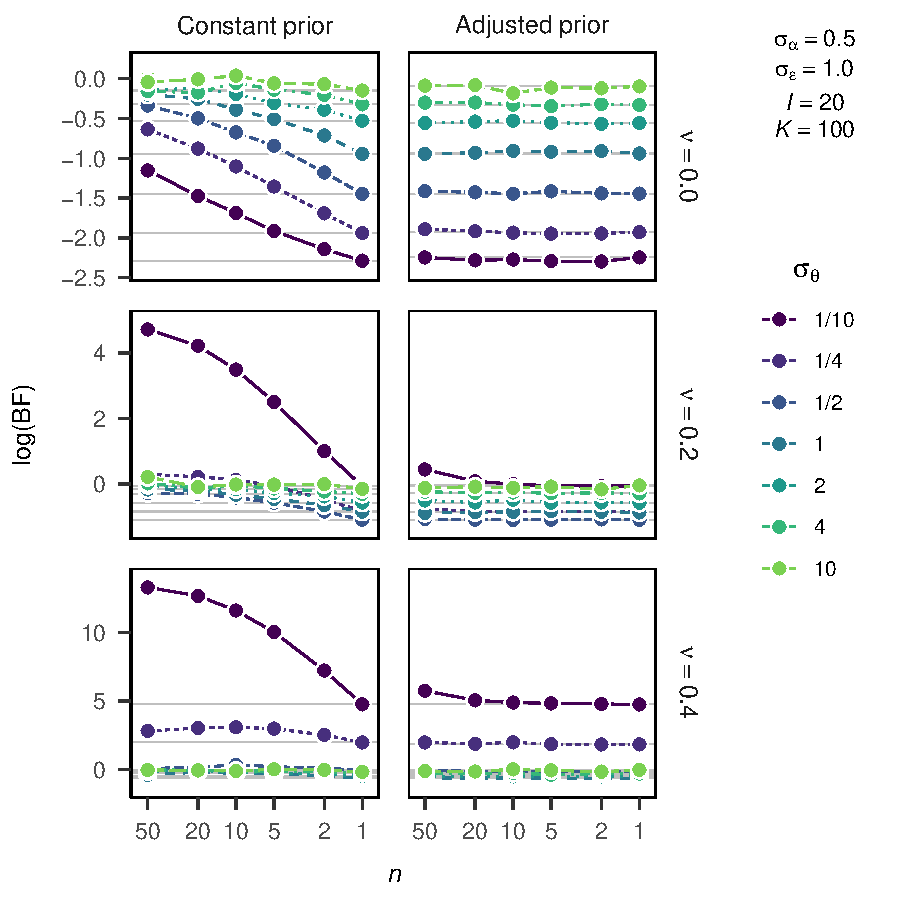
\includegraphics{/Users/frederikaust/Documents/projects/bf-defprit/report/prior_translation_man_files/figure-latex/partial-aggregation-results-1.pdf}
\caption{\label{fig:partial-aggregation-results}Horizontal lines represent \(\log{\mathrm{BF}}\) for each level of \(\sigma_\theta\) with \(n = 1\) (no aggregation) as reference. \(\nu\) denotes the effect size, \(\sigma_\alpha\) the random slopes variance, \(\sigma_\theta\) the random slopes variance, \(\sigma_\epsilon\) the error variance, and \(I\) the number of participants, and \(K\) the number of trials before aggregation.}
\end{figure}

Our results confirm that the prior adjustment works reasonably well, Figure~\ref{fig:partial-aggregation-results}.
However, when an effect was present, the random slope variance \(\sigma_\theta^2\) was substantially smaller than the error variance \(\sigma_\epsilon^2\), and when only two observations per cell remained, we found Bayes factors to be inflated.
This inflation, however, was negligible for small and inconsequential for large Bayes factors.
Thus, in most cases the adjustment of priors for partial aggregation is simple and effective.

\hypertarget{complete-aggregation}{%
\section{Complete aggregation}\label{complete-aggregation}}

Adjusting priors for complete aggregation is more challenging.
When data are fully aggregated data (i.e., \(n = K\)), the random slopes variance \(\sigma_\theta^2\) becomes confounded with the error variance \(\sigma_\epsilon^2\).
In mixed models the random slope variance is characterized by a probability distribution, which prohibits an exact adjustment of the prior by a simple scaling constant.
Here, we explore the adequacy of an approximate adjustment using a point value for the random slope variance.

When aggregating each participant's data to a single observation per cell, the data can analyzed in two ways: By modeling participants' (1) cell means using a one-way repeated-measures ANOVA, or by modeling participants' (2) cell mean differences using a paired \(t\)-test.

\hypertarget{repeated-measures-anova}{%
\subsection{Repeated-measures ANOVA}\label{repeated-measures-anova}}

Aggregation reduces the maximal model to the following,

\[
\begin{aligned}
\bar{y}_{ij\cdot} & \sim \mathcal{N}(\mu + \sigma\prime_\epsilon (\alpha\prime_i + x_j \nu\prime), \sigma\prime_\epsilon^2 + \sigma_\theta^2/2) \\
\alpha\prime_i & \sim \mathcal{N}(0, g_\alpha \sqrt{\sigma_\theta^2}) \\
\nu\prime & \sim \mathcal{N}(0, g_{\nu} \sqrt{\sigma_\theta^2/2}), 
\end{aligned}
\]

where \(x_j\) is an indicates the condition using orthonormal effect coding, \(\pm \sqrt{2}/2\); the random slopes variance \(\sigma_\theta^2\) is scaled by the coding used for \(x_j\).

Compared to partial aggregation, the adjustment for the fixed effect requires an additional factor that depends on a weighted ratio of random variance \(\sigma^2_\theta\) and error variance \(\sigma^2_\epsilon\),

\[
\begin{aligned}
\sqrt{\sigma_\epsilon^2/K + \sigma_\theta^2/2} & = \sigma_\epsilon/\sqrt{K} \sqrt{1 + \frac{K\sigma^2_\theta}{2\sigma_\epsilon^2}} \\
  & = \sigma_\epsilon/\sqrt{K} \sqrt{\frac{2\sigma_\epsilon^2 + K\sigma^2_\theta}{2\sigma_\epsilon^2}} \\
  & = \sigma_\epsilon/\sqrt{K} \sqrt{\frac{2/K + \sigma^2_\theta/\sigma_\epsilon^2}{2/K}} \\
\end{aligned}
\]

For random intercepts, the additional correction factor is obtained by marginalizing over the dummy coded random effect, yielding a weight of 1 for the random slope variance.

\hypertarget{t-test}{%
\subsection{\texorpdfstring{\(t\)-Test}{t-Test}}\label{t-test}}

When analyzing participants' cell mean differences, the random intercept variance cancels out and requires no prior or adjustment.
The prior adjustment for the fixed effect, however, must account for the different effect coding schemes, i.e.~\(\pm 0.5\) vs.~\(\pm \sqrt{2}/2\),

\[
\begin{aligned}
\bar{y}_{ij\cdot} - \bar{y}_{ij\cdot} & \sim \mathcal{N}(\mu + \sigma\prime_\epsilon (\alpha_i + 0.5 \nu), \sigma\prime_\epsilon^2) \\
& - \mathcal{N}(\mu + \sigma\prime_\epsilon (\alpha_i - 0.5 \nu), \sigma\prime_\epsilon^2) \\
  & = \mathcal{N}(\sigma\prime_\epsilon \nu, 2\sigma\prime_\epsilon^2) \\ & \\
  \nu & \sim \mathcal{N}(0, g_\nu \sqrt{\sigma_\theta^2/4}).
\end{aligned}
\]

Rescaling the prior on \(\nu\) to the orthonormal scale, \(\sqrt{2}\nu\), yields the same adjustment as for the prior in the repeated-measures ANOVA,

\[
\begin{aligned}
\sqrt{\sigma_\epsilon^2/K + \sigma_\theta^2/2} & = \sigma_\epsilon/\sqrt{K} \sqrt{1 + \frac{K\sigma^2_\theta}{2\sigma_\epsilon^2}} \\
  & = \sigma_\epsilon/\sqrt{K} \sqrt{\frac{2\sigma_\epsilon^2 + K\sigma^2_\theta}{2\sigma_\epsilon^2}} \\
  & = \sigma_\epsilon/\sqrt{K} \sqrt{\frac{2/K + \sigma^2_\theta/\sigma_\epsilon^2}{2/K}}. \\
\end{aligned}
\]

As noted above in the linear mixed model \(\sigma_\theta^2\) is characterized by a probability distribution.
To test whether the exact adjustment can be approximated by using a point value in the equation above, we conducted a second simulation.

\hypertarget{simulation-1}{%
\subsection{Simulation}\label{simulation-1}}

We randomly simulated \(K = \{5, 25, 100\}\) responses for \(I = \{20, 50, 100, 200\}\) participants (\(\mu = 1\); \(\sigma_\alpha = 0.50\); \(\nu = \{0, 0.2, 0.5\}\); \(\sigma_\theta = 0.50\); \(\sigma_\epsilon = \{0.1, 0.25, 0.5, 1, 2\}\)) 10 times each.
We analyzed the data using mixed models and conducted corresponding repeated-measures ANOVA and paired \(t\)-test as aggregate analyses.
Again, Bayes factors quantify evidence for the maximal model against a model that omits the fixed effect of condition, \(\nu = 0\).

\hypertarget{results-1}{%
\subsubsection{Results}\label{results-1}}



\begin{figure}
\centering
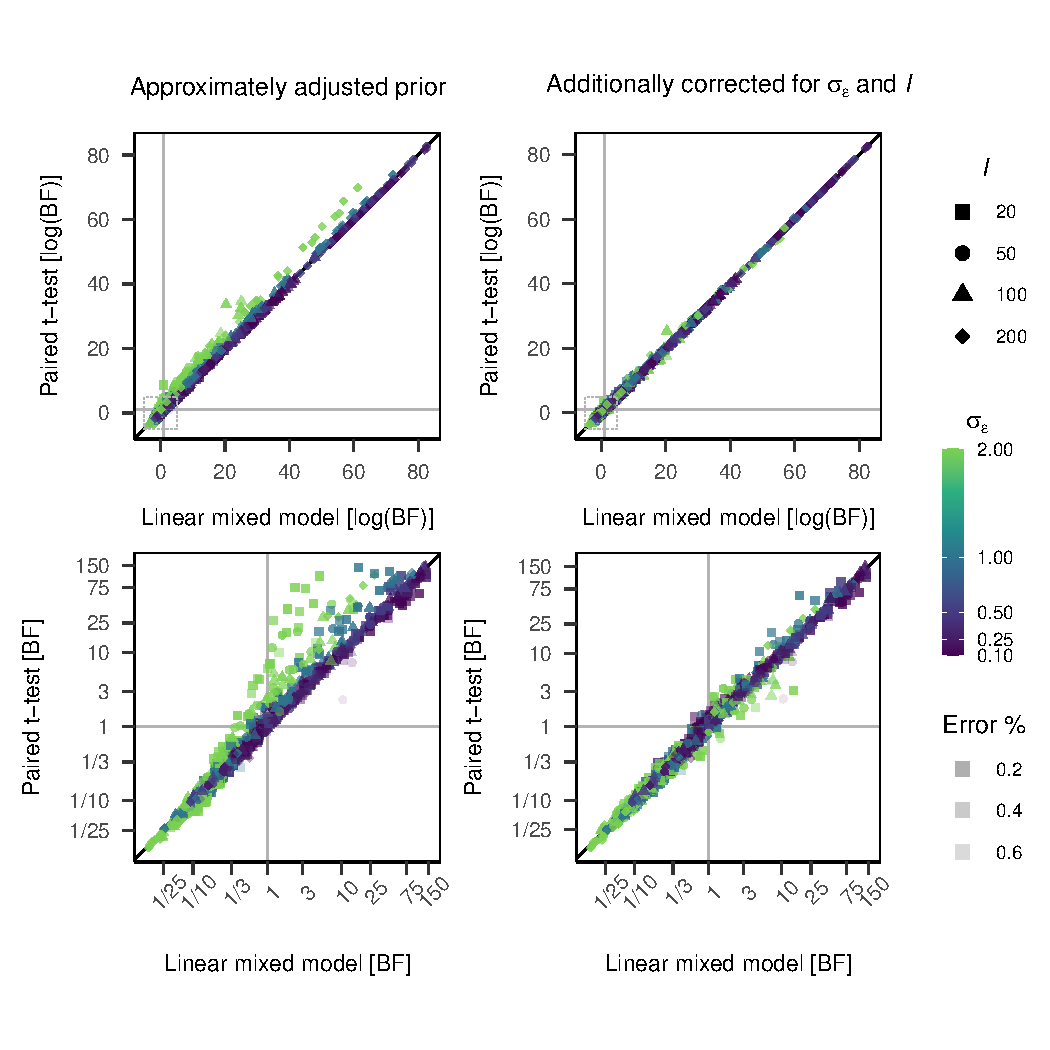
\includegraphics{/Users/frederikaust/Documents/projects/bf-defprit/report/prior_translation_man_files/figure-latex/adjustment-correction-comparison-ttest-1.pdf}
\caption{\label{fig:adjustment-correction-comparison-ttest}Simulation results showing the effect of the approximate adjustment of the prior scale in paired \(t\)-tests on Bayes factors compared to the corresponding mixed model (left) and an additional correction of those Bayes factors by error variance \(\sigma_\epsilon^2\) and number of participants \(I\). The transparency of points represents the reciprocal of the estimation error for mixed model Bayes factors (log scale). The grey dotted square (top) highlights the portion of the plot that is shown in more detail in the bottom panels.}
\end{figure}



\begin{figure}
\centering
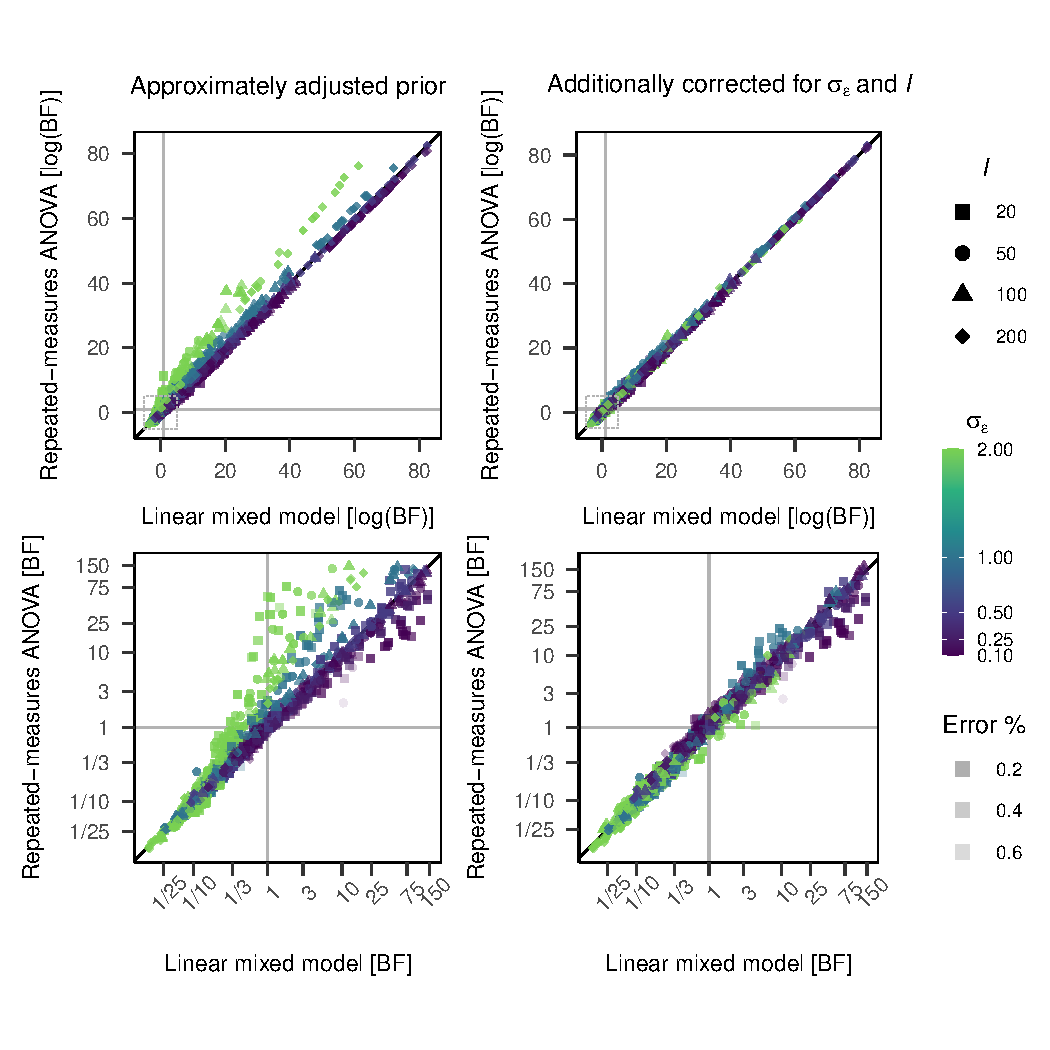
\includegraphics{/Users/frederikaust/Documents/projects/bf-defprit/report/prior_translation_man_files/figure-latex/adjustment-correction-comparison-anova-1.pdf}
\caption{\label{fig:adjustment-correction-comparison-anova}Simulation results showing the effect of the approximate adjustment of the prior scale in repeated-measures ANOVAS on Bayes factors compared to the corresponding mixed model (left) and an additional correction of those Bayes factors by error variance \(\sigma_\epsilon^2\) and number of participants \(I\). The transparency of points represents the reciprocal of the estimation error for mixed model Bayes factors (log scale). The grey dotted square (top) highlights the portion of the plot that is shown in more detail in the bottom panels.}
\end{figure}

When the error variance \(\sigma_\epsilon^2\) was small or the sample size \(I\) was large, the adjustments worked reasonably well, left panels of Figures~\ref{fig:adjustment-correction-comparison-ttest} and \ref{fig:adjustment-correction-comparison-anova}.
However, compared to the mixed model, in many cases both aggregate analyses produced substantially diverging Bayes factors.
The divergence increased as (1) the difference in random slope and error variance increased and (2) the number of participants decreased.
For a detailed breakdown of the results by all varied factors see the online supplementary material at \url{https://github.com/crsh/bf-defprit/}.
The divergence of Bayes factors was more pronounced in the repeated-measures ANOVA than in the paired \(t\)-test, because priors on both fixed and random intercepts require adjustment.

In an exploratory analysis of the simulation results, we compared several regression models (using AIC and BIC) that expressed the Bayes factors from the mixed model (weighted by the reciprocal of their estimation error) as a function of Bayes factors from the corresponding paired \(t\)-test, sample size \(I\), and error variance \(\sigma_\epsilon^2\).
For details refer to the online supplementary material at \url{https://github.com/crsh/bf-defprit/}.
Next, we compared the same set of models for the Bayes factors from repeated-measures ANOVA and found the same winning model.
The Bayes factors predicted by the selected model,

\[
\begin{aligned}
\log\mathrm{BF_{LMM}} = & ~ b_1 \sigma_\epsilon + b_2 \sqrt{\sigma_\epsilon} + b_3 \sqrt{I} + b_4 \sqrt{I} \sigma_\epsilon +\\
    & ~\log \mathrm{BF} (1 + b_5 \sigma_\epsilon^2 + b_6 \log I + b_7 \sigma_\epsilon^2 \log I),
\end{aligned}
\]

largely offset divergences between linear mixed model and aggregate analyses, right panels of Figures~\ref{fig:adjustment-correction-comparison-ttest} and \ref{fig:adjustment-correction-comparison-anova}.

\hypertarget{discussion}{%
\section{Discussion}\label{discussion}}

We explored approximate translations of default priors between mixed models, repeated-measures ANOVA, and paired \(t\)-tests to obtain equivalent Bayes factors.
Although these translations worked reasonably well in the case of partial aggregation, they were less successful for complete aggregation.
We are currently working on refined adjustments to eliminate the observed discrepancies between mixed models and the corresponding aggregate analyses.

\newpage

\hypertarget{references}{%
\section{References}\label{references}}

\hypertarget{refs}{}
\begin{CSLReferences}{1}{0}
\leavevmode\vadjust pre{\hypertarget{ref-heck_benefits_2021}{}}%
Heck, D. W., \& Bockting, F. (2021). Benefits of {Bayesian Model Averaging} for {Mixed-Effects Modeling}. \emph{Computational Brain \& Behavior}. \url{https://doi.org/10.1007/s42113-021-00118-x}

\leavevmode\vadjust pre{\hypertarget{ref-rouder2012}{}}%
Rouder, J. N., Morey, R. D., Speckman, P. L., \& Province, J. M. (2012). Default bayes factors for ANOVA designs. \emph{Journal of Mathematical Psychology}, \emph{56}(5), 356--374. \url{https://doi.org/10.1016/j.jmp.2012.08.001}

\leavevmode\vadjust pre{\hypertarget{ref-singmann_statistics_2022}{}}%
Singmann, H., Kellen, D., Cox, G. E., Chandramouli, S. H., Davis-Stober, C. P., Dunn, J. C., \ldots{} Shiffrin, R. M. (2022). Statistics in the {Service} of {Science}: {Don}'t {Let} the {Tail Wag} the {Dog}. \emph{Computational Brain \& Behavior}. \url{https://doi.org/10.1007/s42113-022-00129-2}

\leavevmode\vadjust pre{\hypertarget{ref-vandoorn2021}{}}%
van Doorn, J., Aust, F., Haaf, J. M., Stefan, A. M., \& Wagenmakers, E.-J. (2021). Bayes factors for mixed models. \emph{Computational Brain \& Behavior}. \url{https://doi.org/10.1007/s42113-021-00113-2}

\end{CSLReferences}


\end{document}
